\documentclass[twoside]{book}

% Packages required by doxygen
\usepackage{fixltx2e}
\usepackage{calc}
\usepackage{doxygen}
\usepackage[export]{adjustbox} % also loads graphicx
\usepackage{graphicx}
\usepackage[utf8]{inputenc}
\usepackage{makeidx}
\usepackage{multicol}
\usepackage{multirow}
\PassOptionsToPackage{warn}{textcomp}
\usepackage{textcomp}
\usepackage[nointegrals]{wasysym}
\usepackage[table]{xcolor}

% Font selection
\usepackage[T1]{fontenc}
\usepackage[scaled=.90]{helvet}
\usepackage{courier}
\usepackage{amssymb}
\usepackage{sectsty}
\renewcommand{\familydefault}{\sfdefault}
\allsectionsfont{%
  \fontseries{bc}\selectfont%
  \color{darkgray}%
}
\renewcommand{\DoxyLabelFont}{%
  \fontseries{bc}\selectfont%
  \color{darkgray}%
}
\newcommand{\+}{\discretionary{\mbox{\scriptsize$\hookleftarrow$}}{}{}}

% Page & text layout
\usepackage{geometry}
\geometry{%
  a4paper,%
  top=2.5cm,%
  bottom=2.5cm,%
  left=2.5cm,%
  right=2.5cm%
}
\tolerance=750
\hfuzz=15pt
\hbadness=750
\setlength{\emergencystretch}{15pt}
\setlength{\parindent}{0cm}
\setlength{\parskip}{3ex plus 2ex minus 2ex}
\makeatletter
\renewcommand{\paragraph}{%
  \@startsection{paragraph}{4}{0ex}{-1.0ex}{1.0ex}{%
    \normalfont\normalsize\bfseries\SS@parafont%
  }%
}
\renewcommand{\subparagraph}{%
  \@startsection{subparagraph}{5}{0ex}{-1.0ex}{1.0ex}{%
    \normalfont\normalsize\bfseries\SS@subparafont%
  }%
}
\makeatother

% Headers & footers
\usepackage{fancyhdr}
\pagestyle{fancyplain}
\fancyhead[LE]{\fancyplain{}{\bfseries\thepage}}
\fancyhead[CE]{\fancyplain{}{}}
\fancyhead[RE]{\fancyplain{}{\bfseries\leftmark}}
\fancyhead[LO]{\fancyplain{}{\bfseries\rightmark}}
\fancyhead[CO]{\fancyplain{}{}}
\fancyhead[RO]{\fancyplain{}{\bfseries\thepage}}
\fancyfoot[LE]{\fancyplain{}{}}
\fancyfoot[CE]{\fancyplain{}{}}
\fancyfoot[RE]{\fancyplain{}{\bfseries\scriptsize Generated by Doxygen }}
\fancyfoot[LO]{\fancyplain{}{\bfseries\scriptsize Generated by Doxygen }}
\fancyfoot[CO]{\fancyplain{}{}}
\fancyfoot[RO]{\fancyplain{}{}}
\renewcommand{\footrulewidth}{0.4pt}
\renewcommand{\chaptermark}[1]{%
  \markboth{#1}{}%
}
\renewcommand{\sectionmark}[1]{%
  \markright{\thesection\ #1}%
}

% Indices & bibliography
\usepackage{natbib}
\usepackage[titles]{tocloft}
\setcounter{tocdepth}{3}
\setcounter{secnumdepth}{5}
\makeindex

% Hyperlinks (required, but should be loaded last)
\usepackage{ifpdf}
\ifpdf
  \usepackage[pdftex,pagebackref=true]{hyperref}
\else
  \usepackage[ps2pdf,pagebackref=true]{hyperref}
\fi
\hypersetup{%
  colorlinks=true,%
  linkcolor=blue,%
  citecolor=blue,%
  unicode%
}

% Custom commands
\newcommand{\clearemptydoublepage}{%
  \newpage{\pagestyle{empty}\cleardoublepage}%
}

\usepackage{caption}
\captionsetup{labelsep=space,justification=centering,font={bf},singlelinecheck=off,skip=4pt,position=top}

%===== C O N T E N T S =====

\begin{document}

% Titlepage & ToC
\hypersetup{pageanchor=false,
             bookmarksnumbered=true,
             pdfencoding=unicode
            }
\pagenumbering{alph}
\begin{titlepage}
\vspace*{7cm}
\begin{center}%
{\Large Gaze data }\\
\vspace*{1cm}
{\large Generated by Doxygen 1.8.13}\\
\end{center}
\end{titlepage}
\clearemptydoublepage
\pagenumbering{roman}
\tableofcontents
\clearemptydoublepage
\pagenumbering{arabic}
\hypersetup{pageanchor=true}

%--- Begin generated contents ---
\chapter{Hierarchical Index}
\section{Class Hierarchy}
This inheritance list is sorted roughly, but not completely, alphabetically\+:\begin{DoxyCompactList}
\item \contentsline{section}{C\+Base\+Highlighter}{\pageref{class_c_base_highlighter}}{}
\begin{DoxyCompactList}
\item \contentsline{section}{C\+Base\+B\+Box}{\pageref{class_c_base_b_box}}{}
\begin{DoxyCompactList}
\item \contentsline{section}{C\+B\+Box}{\pageref{class_c_b_box}}{}
\item \contentsline{section}{C\+Image}{\pageref{class_c_image}}{}
\end{DoxyCompactList}
\item \contentsline{section}{C\+Point}{\pageref{class_c_point}}{}
\end{DoxyCompactList}
\item \contentsline{section}{C\+Gaze\+Capture}{\pageref{class_c_gaze_capture}}{}
\item \contentsline{section}{C\+Landmark}{\pageref{class_c_landmark}}{}
\begin{DoxyCompactList}
\item \contentsline{section}{C\+Gaze}{\pageref{class_c_gaze}}{}
\end{DoxyCompactList}
\item \contentsline{section}{C\+Landmark\+Candidate}{\pageref{class_c_landmark_candidate}}{}
\end{DoxyCompactList}

\chapter{Data Structure Index}
\section{Data Structures}
Here are the data structures with brief descriptions\+:\begin{DoxyCompactList}
\item\contentsline{section}{\hyperlink{class_c_base_b_box}{C\+Base\+B\+Box} }{\pageref{class_c_base_b_box}}{}
\item\contentsline{section}{\hyperlink{class_c_base_highlighter}{C\+Base\+Highlighter} }{\pageref{class_c_base_highlighter}}{}
\item\contentsline{section}{\hyperlink{class_c_b_box}{C\+B\+Box} }{\pageref{class_c_b_box}}{}
\item\contentsline{section}{\hyperlink{class_c_gaze}{C\+Gaze} }{\pageref{class_c_gaze}}{}
\item\contentsline{section}{\hyperlink{class_c_gaze_capture}{C\+Gaze\+Capture} }{\pageref{class_c_gaze_capture}}{}
\item\contentsline{section}{\hyperlink{class_c_image}{C\+Image} }{\pageref{class_c_image}}{}
\item\contentsline{section}{\hyperlink{class_c_landmark}{C\+Landmark} }{\pageref{class_c_landmark}}{}
\item\contentsline{section}{\hyperlink{class_c_landmark_candidate}{C\+Landmark\+Candidate} }{\pageref{class_c_landmark_candidate}}{}
\item\contentsline{section}{\hyperlink{class_c_point}{C\+Point} }{\pageref{class_c_point}}{}
\end{DoxyCompactList}

\chapter{Data Structure Documentation}
\hypertarget{class_c_base_b_box}{}\section{C\+Base\+B\+Box Class Reference}
\label{class_c_base_b_box}\index{C\+Base\+B\+Box@{C\+Base\+B\+Box}}
Inheritance diagram for C\+Base\+B\+Box\+:\begin{figure}[H]
\begin{center}
\leavevmode
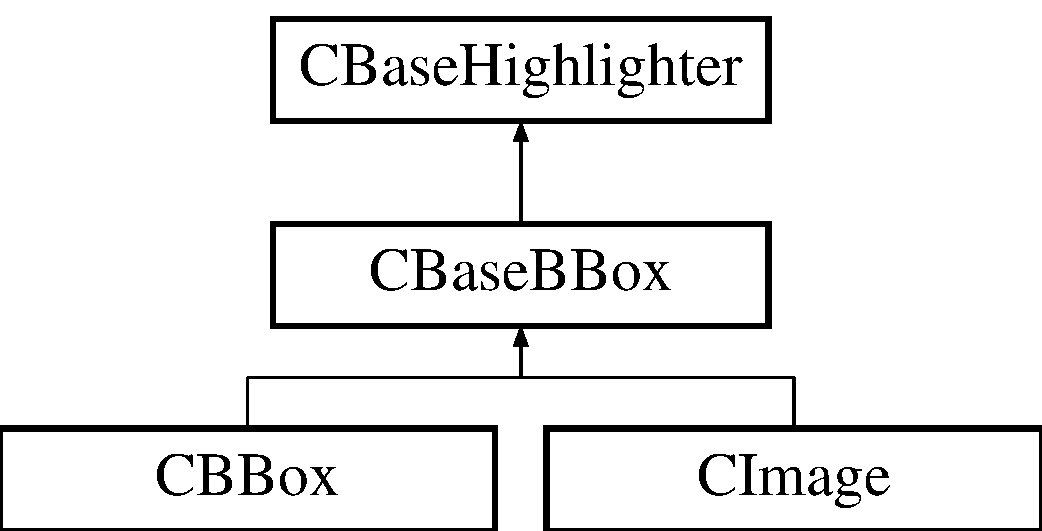
\includegraphics[height=3.000000cm]{class_c_base_b_box}
\end{center}
\end{figure}
\subsection*{Public Member Functions}
\begin{DoxyCompactItemize}
\item 
\mbox{\Hypertarget{class_c_base_b_box_a9e2972e83ca630b10bf61dd5bea2e521}\label{class_c_base_b_box_a9e2972e83ca630b10bf61dd5bea2e521}} 
virtual unsigned int {\bfseries Get\+Width} (unsigned int u\+Level=-\/1) const
\item 
\mbox{\Hypertarget{class_c_base_b_box_ad96488a621c64bb65eb7809b3e882890}\label{class_c_base_b_box_ad96488a621c64bb65eb7809b3e882890}} 
virtual unsigned int {\bfseries Get\+Height} (unsigned int u\+Level=-\/1) const
\item 
\mbox{\Hypertarget{class_c_base_b_box_aa56bf53aae50f5e9bef2356ec34b2e51}\label{class_c_base_b_box_aa56bf53aae50f5e9bef2356ec34b2e51}} 
\hyperlink{class_c_base_b_box}{C\+Base\+B\+Box} $\ast$ {\bfseries Get\+Parent} (unsigned int u\+Level=-\/1) override
\item 
\mbox{\Hypertarget{class_c_base_b_box_ae71c6114cb963709bc843c871f51093a}\label{class_c_base_b_box_ae71c6114cb963709bc843c871f51093a}} 
virtual void {\bfseries Transfer\+Ownership} (unsigned int u\+Level=1)
\item 
\mbox{\Hypertarget{class_c_base_b_box_a5baea44b1a2a9c18f8edddf8d6e1a365}\label{class_c_base_b_box_a5baea44b1a2a9c18f8edddf8d6e1a365}} 
virtual void {\bfseries Transfer\+Ownership} (\hyperlink{class_c_base_b_box}{C\+Base\+B\+Box} \&parent\+Box)
\end{DoxyCompactItemize}
\subsection*{Protected Member Functions}
\begin{DoxyCompactItemize}
\item 
\mbox{\Hypertarget{class_c_base_b_box_a98aeefbd3d2a5d3fddbff2a15a1f926d}\label{class_c_base_b_box_a98aeefbd3d2a5d3fddbff2a15a1f926d}} 
{\bfseries C\+Base\+B\+Box} (const char $\ast$sz\+Name)
\item 
\mbox{\Hypertarget{class_c_base_b_box_a7f317d3b2721d89328cedb18afbd910e}\label{class_c_base_b_box_a7f317d3b2721d89328cedb18afbd910e}} 
{\bfseries C\+Base\+B\+Box} (const \hyperlink{class_c_base_b_box}{C\+Base\+B\+Box} \&other)
\item 
\mbox{\Hypertarget{class_c_base_b_box_a8c82f37c693b3c771e1fe3c43b932059}\label{class_c_base_b_box_a8c82f37c693b3c771e1fe3c43b932059}} 
{\bfseries C\+Base\+B\+Box} (\hyperlink{class_c_base_b_box}{C\+Base\+B\+Box} \&parent\+Box, unsigned int uX, unsigned int uY, unsigned int u\+Width, unsigned int u\+Height, unsigned int u\+Level, const char $\ast$sz\+Name)
\item 
\mbox{\Hypertarget{class_c_base_b_box_abdee10baefbacc0376572f31f1c8416c}\label{class_c_base_b_box_abdee10baefbacc0376572f31f1c8416c}} 
{\bfseries C\+Base\+B\+Box} (\hyperlink{class_c_base_b_box}{C\+Base\+B\+Box} \&parent\+Box, double dX, double dY, double d\+Width, double d\+Height, const char $\ast$sz\+Name)
\item 
\mbox{\Hypertarget{class_c_base_b_box_ac98ee8da50886c5b8e74fcbe1130abc4}\label{class_c_base_b_box_ac98ee8da50886c5b8e74fcbe1130abc4}} 
void {\bfseries Swap} (\hyperlink{class_c_base_b_box}{C\+Base\+B\+Box} \&other, bool f\+Swap\+Children=true)
\end{DoxyCompactItemize}
\subsection*{Protected Attributes}
\begin{DoxyCompactItemize}
\item 
\mbox{\Hypertarget{class_c_base_b_box_abc694b352766ffc4902c4fd2b8cc978a}\label{class_c_base_b_box_abc694b352766ffc4902c4fd2b8cc978a}} 
double {\bfseries m\+\_\+d\+Width} = 1
\item 
\mbox{\Hypertarget{class_c_base_b_box_a24ab993e6da60fa3a1d67f21a2784e86}\label{class_c_base_b_box_a24ab993e6da60fa3a1d67f21a2784e86}} 
double \hyperlink{class_c_base_b_box_a24ab993e6da60fa3a1d67f21a2784e86}{m\+\_\+d\+Height} = 1
\begin{DoxyCompactList}\small\item\em Width in \% of parent\textquotesingle{}s width. \end{DoxyCompactList}\item 
\mbox{\Hypertarget{class_c_base_b_box_a7c5d97459f753e92bfa34497294683f4}\label{class_c_base_b_box_a7c5d97459f753e92bfa34497294683f4}} 
friend \hyperlink{class_c_base_b_box_a7c5d97459f753e92bfa34497294683f4}{C\+Base\+Highlighter}
\begin{DoxyCompactList}\small\item\em Height in \% of parent\textquotesingle{}s height. \end{DoxyCompactList}\end{DoxyCompactItemize}
\subsection*{Additional Inherited Members}


The documentation for this class was generated from the following files\+:\begin{DoxyCompactItemize}
\item 
D\+:/\+Users/\+Rainer/\+Source/\+Repos/deep\+\_\+learning/gaze\+\_\+data/Base\+B\+Box.\+h\item 
D\+:/\+Users/\+Rainer/\+Source/\+Repos/deep\+\_\+learning/gaze\+\_\+data/Base\+B\+Box.\+cpp\end{DoxyCompactItemize}

\hypertarget{class_c_base_highlighter}{}\section{C\+Base\+Highlighter Class Reference}
\label{class_c_base_highlighter}\index{C\+Base\+Highlighter@{C\+Base\+Highlighter}}
Inheritance diagram for C\+Base\+Highlighter\+:\begin{figure}[H]
\begin{center}
\leavevmode
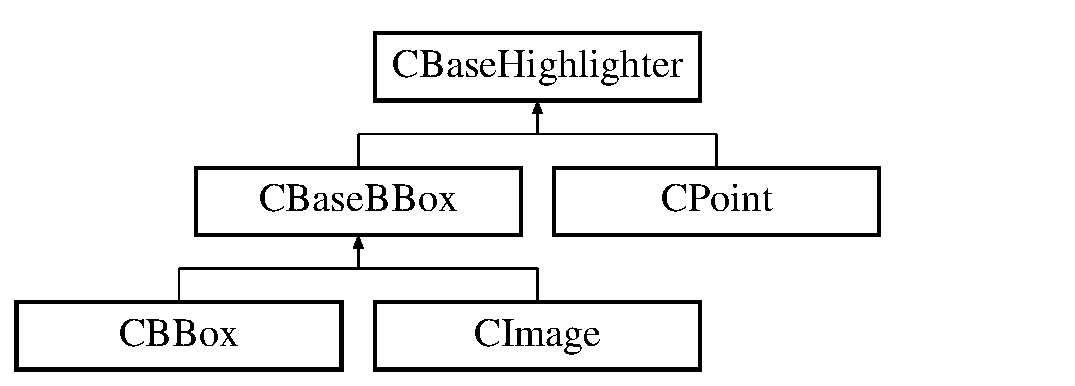
\includegraphics[height=3.000000cm]{class_c_base_highlighter}
\end{center}
\end{figure}
\subsection*{Public Member Functions}
\begin{DoxyCompactItemize}
\item 
\mbox{\Hypertarget{class_c_base_highlighter_acd04321a5f64f77d59a37a2f0ca235fb}\label{class_c_base_highlighter_acd04321a5f64f77d59a37a2f0ca235fb}} 
virtual unsigned int {\bfseries Get\+PositionX} (unsigned int u\+Level=-\/1) const
\item 
\mbox{\Hypertarget{class_c_base_highlighter_a382ec7cbb665e220dedc4473d6725998}\label{class_c_base_highlighter_a382ec7cbb665e220dedc4473d6725998}} 
virtual unsigned int {\bfseries Get\+PositionY} (unsigned int u\+Level=-\/1) const
\item 
\mbox{\Hypertarget{class_c_base_highlighter_a770796fc3ef5afe56b71ea02f711740d}\label{class_c_base_highlighter_a770796fc3ef5afe56b71ea02f711740d}} 
virtual \hyperlink{class_c_image}{C\+Image} $\ast$ {\bfseries Get\+Image} (unsigned int u\+Level=-\/1)
\item 
\mbox{\Hypertarget{class_c_base_highlighter_a6d1d5b8b30a52c78bc50e3968a0d7907}\label{class_c_base_highlighter_a6d1d5b8b30a52c78bc50e3968a0d7907}} 
virtual \hyperlink{class_c_base_b_box}{C\+Base\+B\+Box} $\ast$ {\bfseries Get\+Parent} (unsigned int u\+Level=-\/1)
\item 
\mbox{\Hypertarget{class_c_base_highlighter_a72f841d27775ea6d9a32279748490e90}\label{class_c_base_highlighter_a72f841d27775ea6d9a32279748490e90}} 
virtual void {\bfseries Transfer\+Ownership} (unsigned int u\+Level=1)
\item 
\mbox{\Hypertarget{class_c_base_highlighter_a23bdfc98cb2cffc9f3125d34f77c31fa}\label{class_c_base_highlighter_a23bdfc98cb2cffc9f3125d34f77c31fa}} 
virtual void {\bfseries Transfer\+Ownership} (\hyperlink{class_c_base_b_box}{C\+Base\+B\+Box} \&parent\+Box)
\end{DoxyCompactItemize}
\subsection*{Data Fields}
\begin{DoxyCompactItemize}
\item 
\mbox{\Hypertarget{class_c_base_highlighter_a8602a164489e2650d8871ec43b155876}\label{class_c_base_highlighter_a8602a164489e2650d8871ec43b155876}} 
const char {\bfseries sz\+Name} \mbox{[}32\mbox{]}
\end{DoxyCompactItemize}
\subsection*{Protected Member Functions}
\begin{DoxyCompactItemize}
\item 
\mbox{\Hypertarget{class_c_base_highlighter_aca6eda19fca9586f96375cdedee59aba}\label{class_c_base_highlighter_aca6eda19fca9586f96375cdedee59aba}} 
{\bfseries C\+Base\+Highlighter} (const char $\ast$sz\+Name)
\item 
\mbox{\Hypertarget{class_c_base_highlighter_ab833e2c0d622fc91eda9e61573b426fa}\label{class_c_base_highlighter_ab833e2c0d622fc91eda9e61573b426fa}} 
{\bfseries C\+Base\+Highlighter} (\hyperlink{class_c_base_b_box}{C\+Base\+B\+Box} \&parent\+Box, unsigned int uX, unsigned int uY, unsigned int u\+Level, const char $\ast$sz\+Name)
\item 
\mbox{\Hypertarget{class_c_base_highlighter_a9101fe0276c64b2fc68287c36e972ddb}\label{class_c_base_highlighter_a9101fe0276c64b2fc68287c36e972ddb}} 
{\bfseries C\+Base\+Highlighter} (\hyperlink{class_c_base_b_box}{C\+Base\+B\+Box} \&parent\+Box, double dX, double dY, const char $\ast$sz\+Name)
\item 
\mbox{\Hypertarget{class_c_base_highlighter_a48b5457668dbf9a5a3bd706b87374bc0}\label{class_c_base_highlighter_a48b5457668dbf9a5a3bd706b87374bc0}} 
{\bfseries C\+Base\+Highlighter} (const \hyperlink{class_c_base_highlighter}{C\+Base\+Highlighter} \&other)
\item 
\mbox{\Hypertarget{class_c_base_highlighter_a984659e2d593fbcf5517c3ef100a24c1}\label{class_c_base_highlighter_a984659e2d593fbcf5517c3ef100a24c1}} 
void {\bfseries Swap} (\hyperlink{class_c_base_highlighter}{C\+Base\+Highlighter} \&other, bool f\+Swap\+Children=true)
\item 
\mbox{\Hypertarget{class_c_base_highlighter_a2774da903ea3e43a6170dee3dd7527f9}\label{class_c_base_highlighter_a2774da903ea3e43a6170dee3dd7527f9}} 
void {\bfseries Add\+Child} (\hyperlink{class_c_base_highlighter}{C\+Base\+Highlighter} $\ast$p\+Child)
\item 
\mbox{\Hypertarget{class_c_base_highlighter_ae15824495f2c80820dcbc6d460e2a411}\label{class_c_base_highlighter_ae15824495f2c80820dcbc6d460e2a411}} 
bool {\bfseries Remove\+Child} (\hyperlink{class_c_base_highlighter}{C\+Base\+Highlighter} $\ast$p\+Child)
\end{DoxyCompactItemize}
\subsection*{Protected Attributes}
\begin{DoxyCompactItemize}
\item 
\mbox{\Hypertarget{class_c_base_highlighter_a50d2c04e5cea521c2973736d05bf6fc9}\label{class_c_base_highlighter_a50d2c04e5cea521c2973736d05bf6fc9}} 
\hyperlink{class_c_base_b_box}{C\+Base\+B\+Box} $\ast$ {\bfseries m\+\_\+p\+Parent\+Box}
\item 
\mbox{\Hypertarget{class_c_base_highlighter_ad58879d75792699960746b0ee3730b51}\label{class_c_base_highlighter_ad58879d75792699960746b0ee3730b51}} 
std\+::vector$<$ \hyperlink{class_c_base_highlighter}{C\+Base\+Highlighter} $\ast$ $>$ {\bfseries m\+\_\+vecp\+Children}
\item 
\mbox{\Hypertarget{class_c_base_highlighter_ab01e3e5c513dcf32c344d7f775c93638}\label{class_c_base_highlighter_ab01e3e5c513dcf32c344d7f775c93638}} 
double {\bfseries m\+\_\+d\+PositionX} = 0
\item 
\mbox{\Hypertarget{class_c_base_highlighter_a53f8a33847b74f021585eb1009ee0b33}\label{class_c_base_highlighter_a53f8a33847b74f021585eb1009ee0b33}} 
double {\bfseries m\+\_\+d\+PositionY} = 0
\end{DoxyCompactItemize}


The documentation for this class was generated from the following files\+:\begin{DoxyCompactItemize}
\item 
D\+:/\+Users/\+Rainer/\+Source/\+Repos/deep\+\_\+learning/gaze\+\_\+data/Base\+Highlighter.\+h\item 
D\+:/\+Users/\+Rainer/\+Source/\+Repos/deep\+\_\+learning/gaze\+\_\+data/Base\+Highlighter.\+cpp\end{DoxyCompactItemize}

\hypertarget{class_c_b_box}{}\section{C\+B\+Box Class Reference}
\label{class_c_b_box}\index{C\+B\+Box@{C\+B\+Box}}
Inheritance diagram for C\+B\+Box\+:\begin{figure}[H]
\begin{center}
\leavevmode
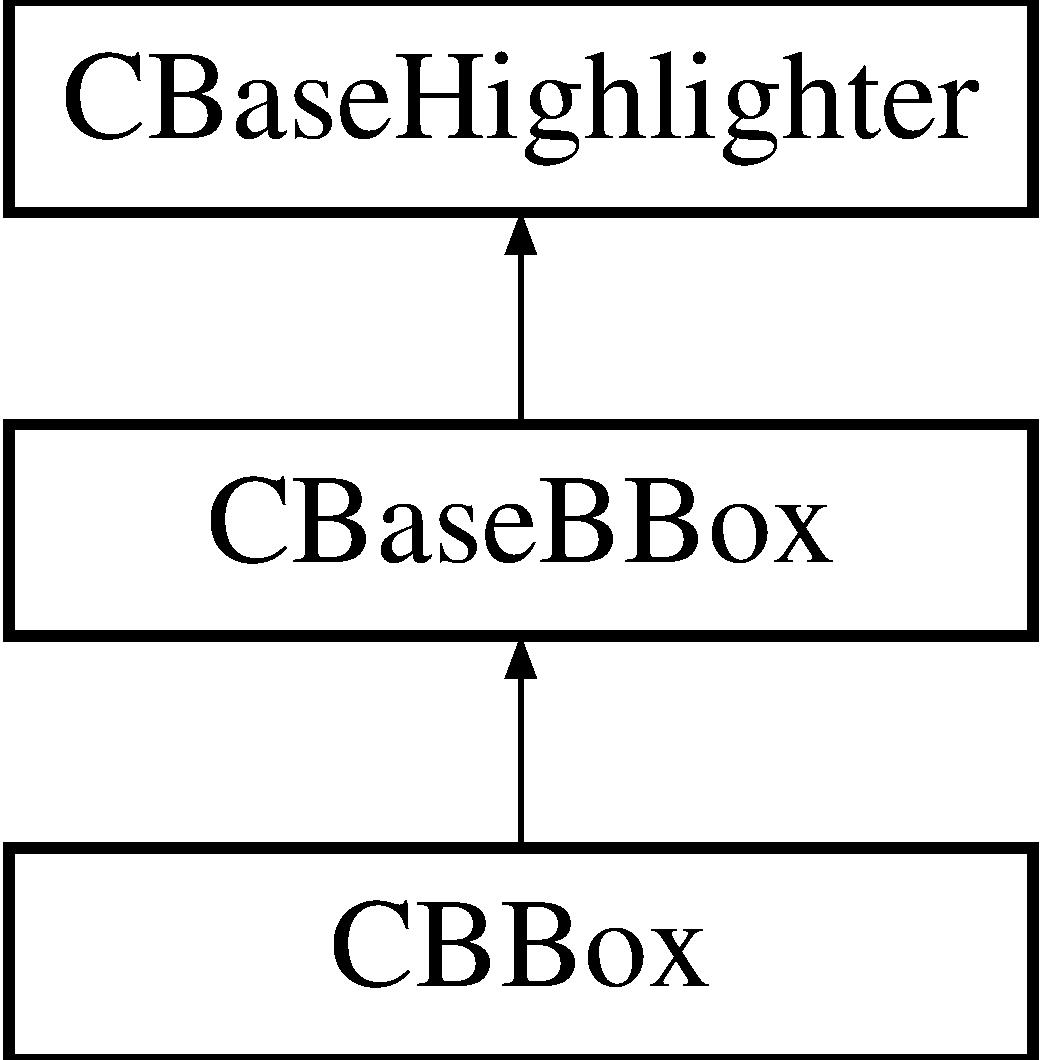
\includegraphics[height=3.000000cm]{class_c_b_box}
\end{center}
\end{figure}
\subsection*{Public Member Functions}
\begin{DoxyCompactItemize}
\item 
\mbox{\Hypertarget{class_c_b_box_acbc98a4ce72444658d4adcc1a86944b5}\label{class_c_b_box_acbc98a4ce72444658d4adcc1a86944b5}} 
{\bfseries C\+B\+Box} (\hyperlink{class_c_base_b_box}{C\+Base\+B\+Box} \&parent\+Box, const cv\+::\+Rect \&rect, unsigned int u\+Level, const char $\ast$sz\+Name)
\item 
\mbox{\Hypertarget{class_c_b_box_a2cab53d1fa862cdafbf8a73d35336344}\label{class_c_b_box_a2cab53d1fa862cdafbf8a73d35336344}} 
{\bfseries C\+B\+Box} (const \hyperlink{class_c_b_box}{C\+B\+Box} \&other)
\item 
\mbox{\Hypertarget{class_c_b_box_a9fa5731118363787c5e979798c27b924}\label{class_c_b_box_a9fa5731118363787c5e979798c27b924}} 
void {\bfseries Swap} (\hyperlink{class_c_b_box}{C\+B\+Box} \&other, bool f\+Swap\+Children=true)
\item 
\mbox{\Hypertarget{class_c_b_box_a61f274eb6091494a6fb6b1497c975919}\label{class_c_b_box_a61f274eb6091494a6fb6b1497c975919}} 
\hyperlink{class_c_b_box}{C\+B\+Box} \& {\bfseries operator=} (const \hyperlink{class_c_b_box}{C\+B\+Box} \&other)
\item 
\mbox{\Hypertarget{class_c_b_box_a7d39f53184eb6d21df0816be7e104a13}\label{class_c_b_box_a7d39f53184eb6d21df0816be7e104a13}} 
void {\bfseries Draw} (const cv\+::\+Scalar \&color, int i\+Thickness=2, unsigned int u\+Level=-\/1)
\item 
\mbox{\Hypertarget{class_c_b_box_a480b8b1e36efb75aa76e8d90437b816e}\label{class_c_b_box_a480b8b1e36efb75aa76e8d90437b816e}} 
void {\bfseries Draw} (\hyperlink{class_c_image}{C\+Image} \&img, const cv\+::\+Scalar \&color, int i\+Thickness=2)
\end{DoxyCompactItemize}
\subsection*{Additional Inherited Members}


The documentation for this class was generated from the following files\+:\begin{DoxyCompactItemize}
\item 
D\+:/\+Users/\+Rainer/\+Source/\+Repos/deep\+\_\+learning/gaze\+\_\+data/B\+Box.\+h\item 
D\+:/\+Users/\+Rainer/\+Source/\+Repos/deep\+\_\+learning/gaze\+\_\+data/B\+Box.\+cpp\end{DoxyCompactItemize}

\hypertarget{class_c_gaze}{}\section{C\+Gaze Class Reference}
\label{class_c_gaze}\index{C\+Gaze@{C\+Gaze}}
Inheritance diagram for C\+Gaze\+:\begin{figure}[H]
\begin{center}
\leavevmode
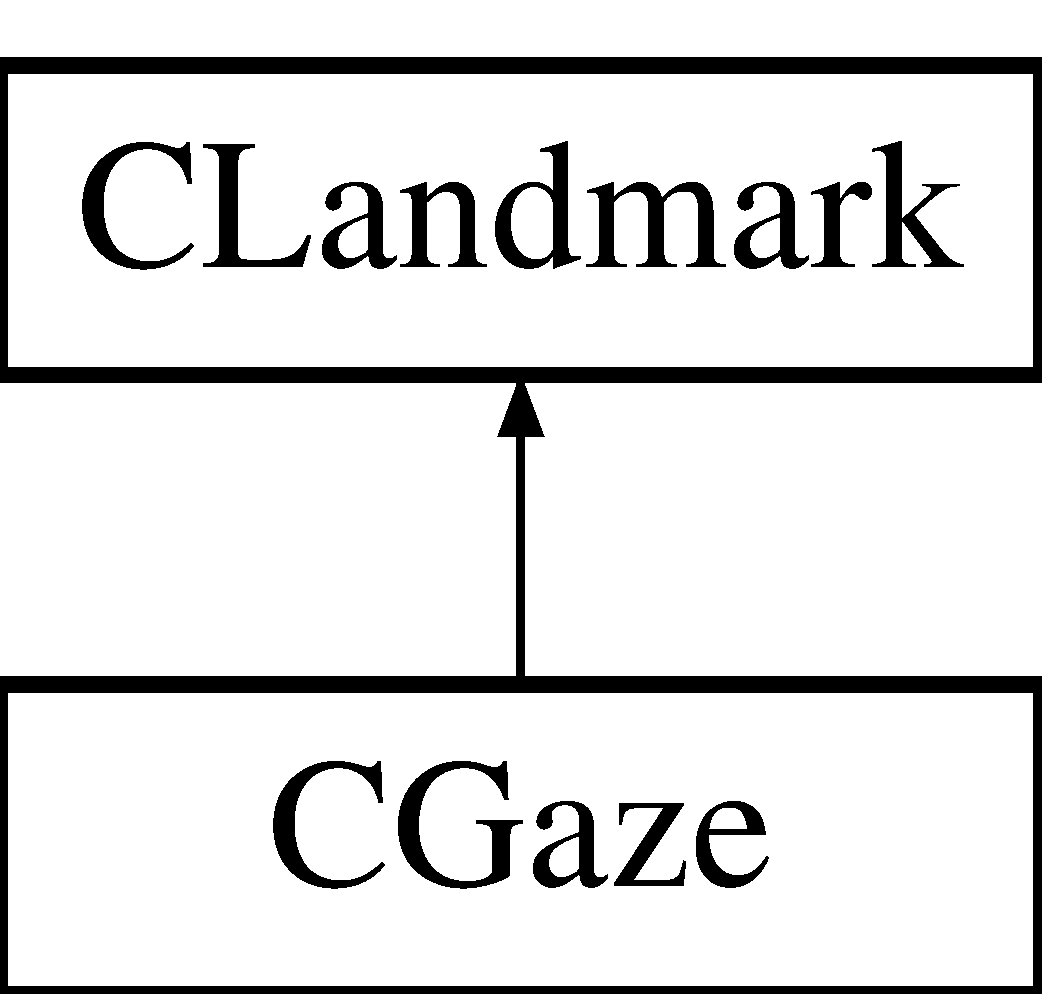
\includegraphics[height=2.000000cm]{class_c_gaze}
\end{center}
\end{figure}
\subsection*{Additional Inherited Members}


The documentation for this class was generated from the following file\+:\begin{DoxyCompactItemize}
\item 
D\+:/\+Users/\+Rainer/\+Source/\+Repos/deep\+\_\+learning/gaze\+\_\+data/Gaze.\+h\end{DoxyCompactItemize}

\hypertarget{class_c_gaze_capture}{}\section{C\+Gaze\+Capture Class Reference}
\label{class_c_gaze_capture}\index{C\+Gaze\+Capture@{C\+Gaze\+Capture}}
\subsection*{Public Member Functions}
\begin{DoxyCompactItemize}
\item 
\mbox{\Hypertarget{class_c_gaze_capture_ad6c7d65869605992d64a9c52ae458ccf}\label{class_c_gaze_capture_ad6c7d65869605992d64a9c52ae458ccf}} 
{\bfseries C\+Gaze\+Capture} (cv\+::\+Video\+Capture \&cap, const char $\ast$sz\+Window)
\item 
\mbox{\Hypertarget{class_c_gaze_capture_aadb497c78141d331c0687ba7b9cf21f2}\label{class_c_gaze_capture_aadb497c78141d331c0687ba7b9cf21f2}} 
{\bfseries C\+Gaze\+Capture} (const \hyperlink{class_c_gaze_capture}{C\+Gaze\+Capture} \&other)
\item 
\mbox{\Hypertarget{class_c_gaze_capture_a28f96ebcf50365b96bbd3be84ede256e}\label{class_c_gaze_capture_a28f96ebcf50365b96bbd3be84ede256e}} 
void {\bfseries Swap} (\hyperlink{class_c_gaze_capture}{C\+Gaze\+Capture} \&other, bool f\+Swap\+Children=true)
\item 
\mbox{\Hypertarget{class_c_gaze_capture_a144457f3a900130378bce311b2aea02c}\label{class_c_gaze_capture_a144457f3a900130378bce311b2aea02c}} 
\hyperlink{class_c_gaze_capture}{C\+Gaze\+Capture} \& {\bfseries operator=} (const \hyperlink{class_c_gaze_capture}{C\+Gaze\+Capture} \&other)
\end{DoxyCompactItemize}
\subsection*{Static Public Member Functions}
\begin{DoxyCompactItemize}
\item 
\mbox{\Hypertarget{class_c_gaze_capture_a8686afa20893c8503c0cc400745d1093}\label{class_c_gaze_capture_a8686afa20893c8503c0cc400745d1093}} 
static void {\bfseries Init} (cv\+::\+Video\+Capture \&cap)
\item 
\mbox{\Hypertarget{class_c_gaze_capture_ac70f160475539df0717eef31c8cdc0a6}\label{class_c_gaze_capture_ac70f160475539df0717eef31c8cdc0a6}} 
static void {\bfseries Get\+Screen\+Resolution} (unsigned int \&u\+Width, unsigned int \&u\+Height)
\end{DoxyCompactItemize}
\subsection*{Data Fields}
\begin{DoxyCompactItemize}
\item 
\mbox{\Hypertarget{class_c_gaze_capture_ad466c17d2b1ca4f2ef5f61fbca1faa0a}\label{class_c_gaze_capture_ad466c17d2b1ca4f2ef5f61fbca1faa0a}} 
\hyperlink{class_c_point}{C\+Point} {\bfseries pt\+Gaze}
\item 
\mbox{\Hypertarget{class_c_gaze_capture_a3f3eba32fb105466c73e8c1e5f5e6887}\label{class_c_gaze_capture_a3f3eba32fb105466c73e8c1e5f5e6887}} 
\hyperlink{class_c_image}{C\+Image} {\bfseries img\+Gaze}
\end{DoxyCompactItemize}


The documentation for this class was generated from the following files\+:\begin{DoxyCompactItemize}
\item 
D\+:/\+Users/\+Rainer/\+Source/\+Repos/deep\+\_\+learning/gaze\+\_\+data/Gaze\+Capture.\+h\item 
D\+:/\+Users/\+Rainer/\+Source/\+Repos/deep\+\_\+learning/gaze\+\_\+data/Gaze\+Capture.\+cpp\end{DoxyCompactItemize}

\hypertarget{class_c_image}{}\section{C\+Image Class Reference}
\label{class_c_image}\index{C\+Image@{C\+Image}}
Inheritance diagram for C\+Image\+:\begin{figure}[H]
\begin{center}
\leavevmode
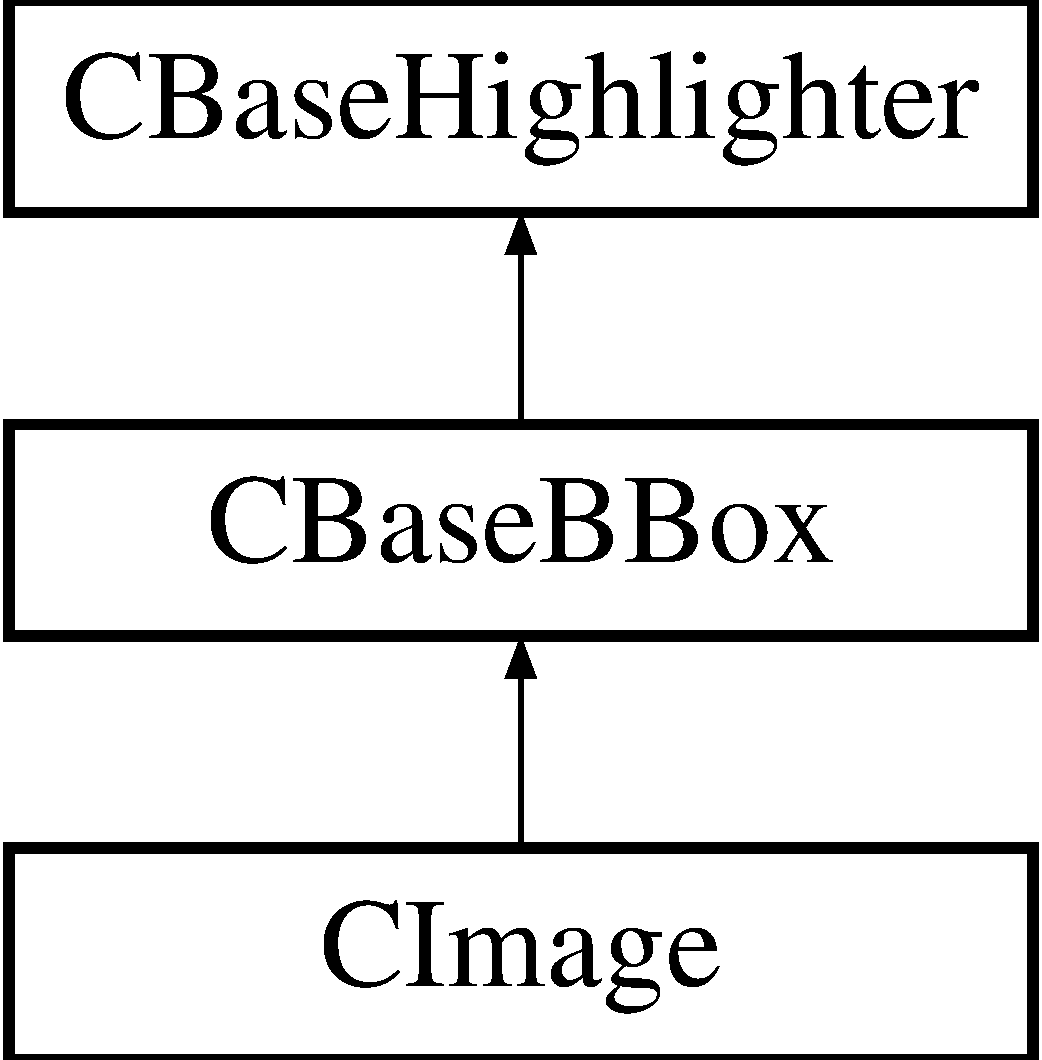
\includegraphics[height=3.000000cm]{class_c_image}
\end{center}
\end{figure}
\subsection*{Public Member Functions}
\begin{DoxyCompactItemize}
\item 
\mbox{\Hypertarget{class_c_image_a21cd70160981d8e10e17be1731bcbadc}\label{class_c_image_a21cd70160981d8e10e17be1731bcbadc}} 
{\bfseries C\+Image} (const char $\ast$sz\+Name)
\item 
\mbox{\Hypertarget{class_c_image_a35bee31efed6acd1a6d35c9554d710ce}\label{class_c_image_a35bee31efed6acd1a6d35c9554d710ce}} 
{\bfseries C\+Image} (cv\+::\+Mat \&mat, const char $\ast$sz\+Name)
\item 
\mbox{\Hypertarget{class_c_image_a8b4314c801dc837e80dd95c0783d2bed}\label{class_c_image_a8b4314c801dc837e80dd95c0783d2bed}} 
{\bfseries C\+Image} (const \hyperlink{class_c_image}{C\+Image} \&other)
\item 
\mbox{\Hypertarget{class_c_image_ac606178f3d62ff9f18fb9d78fb21a0ae}\label{class_c_image_ac606178f3d62ff9f18fb9d78fb21a0ae}} 
{\bfseries C\+Image} (\hyperlink{class_c_image}{C\+Image} \&img, const char $\ast$sz\+Name)
\item 
\mbox{\Hypertarget{class_c_image_a9dbac297b3f353e847d1f681aa616b3f}\label{class_c_image_a9dbac297b3f353e847d1f681aa616b3f}} 
{\bfseries C\+Image} (\hyperlink{class_c_image}{C\+Image} \&parent\+Image, cv\+::\+Mat \&mat\+Image, const cv\+::\+Point \&point, const char $\ast$sz\+Name)
\item 
\mbox{\Hypertarget{class_c_image_a5d51142006c5db5e16760523d82ff284}\label{class_c_image_a5d51142006c5db5e16760523d82ff284}} 
void {\bfseries Swap} (\hyperlink{class_c_image}{C\+Image} \&other, bool f\+Swap\+Children=true)
\item 
\mbox{\Hypertarget{class_c_image_a0ef878c3d788d3db9686e1f2e5bfaaaf}\label{class_c_image_a0ef878c3d788d3db9686e1f2e5bfaaaf}} 
\hyperlink{class_c_image}{C\+Image} \& {\bfseries operator=} (const \hyperlink{class_c_image}{C\+Image} \&other)
\item 
\mbox{\Hypertarget{class_c_image_a22fe91a95249af8ead1325b515986f8a}\label{class_c_image_a22fe91a95249af8ead1325b515986f8a}} 
unsigned int {\bfseries Get\+PositionX} (unsigned int u\+Level=-\/1) const override
\item 
\mbox{\Hypertarget{class_c_image_abfde3dc9e893134cd44d642de9d91d87}\label{class_c_image_abfde3dc9e893134cd44d642de9d91d87}} 
unsigned int {\bfseries Get\+PositionY} (unsigned int u\+Level=-\/1) const override
\item 
\mbox{\Hypertarget{class_c_image_a9a3cb583ae8f174275d23f4e815fb995}\label{class_c_image_a9a3cb583ae8f174275d23f4e815fb995}} 
unsigned int {\bfseries Get\+Width} (unsigned int u\+Level=-\/1) const override
\item 
\mbox{\Hypertarget{class_c_image_a473d570aeb9e1b144cd14b2d811c546e}\label{class_c_image_a473d570aeb9e1b144cd14b2d811c546e}} 
unsigned int {\bfseries Get\+Height} (unsigned int u\+Level=-\/1) const override
\item 
\mbox{\Hypertarget{class_c_image_ad6973a532fcbc6f409406b17c4e850da}\label{class_c_image_ad6973a532fcbc6f409406b17c4e850da}} 
\hyperlink{class_c_image}{C\+Image} $\ast$ {\bfseries Get\+Image} (unsigned int u\+Level=-\/1) override
\item 
\mbox{\Hypertarget{class_c_image_a85ee33c3ecfc97f82bbf7034079d785f}\label{class_c_image_a85ee33c3ecfc97f82bbf7034079d785f}} 
void {\bfseries Transfer\+Ownership} (unsigned int u\+Level=1) override
\item 
\mbox{\Hypertarget{class_c_image_a1add3042a22efb5e828fe786fd98f1de}\label{class_c_image_a1add3042a22efb5e828fe786fd98f1de}} 
void {\bfseries Transfer\+Ownership} (\hyperlink{class_c_base_b_box}{C\+Base\+B\+Box} \&parent\+Box) override
\item 
\mbox{\Hypertarget{class_c_image_a924b9367ed2850ab65ef9e21c09f6366}\label{class_c_image_a924b9367ed2850ab65ef9e21c09f6366}} 
void {\bfseries Show} (const char $\ast$sz\+Window)
\item 
\mbox{\Hypertarget{class_c_image_a47709f5aa2f3d830b6077aec02c5af3a}\label{class_c_image_a47709f5aa2f3d830b6077aec02c5af3a}} 
void {\bfseries Crop} (\hyperlink{class_c_b_box}{C\+B\+Box} \&box, unsigned int u\+Level=0)
\end{DoxyCompactItemize}
\subsection*{Data Fields}
\begin{DoxyCompactItemize}
\item 
\mbox{\Hypertarget{class_c_image_a58684a2b3cfafec2e433018166a21f28}\label{class_c_image_a58684a2b3cfafec2e433018166a21f28}} 
cv\+::\+Mat {\bfseries mat\+Image}
\end{DoxyCompactItemize}
\subsection*{Additional Inherited Members}


The documentation for this class was generated from the following files\+:\begin{DoxyCompactItemize}
\item 
D\+:/\+Users/\+Rainer/\+Source/\+Repos/deep\+\_\+learning/gaze\+\_\+data/Image.\+h\item 
D\+:/\+Users/\+Rainer/\+Source/\+Repos/deep\+\_\+learning/gaze\+\_\+data/Image.\+cpp\end{DoxyCompactItemize}

\hypertarget{class_c_landmark}{}\section{C\+Landmark Class Reference}
\label{class_c_landmark}\index{C\+Landmark@{C\+Landmark}}
Inheritance diagram for C\+Landmark\+:\begin{figure}[H]
\begin{center}
\leavevmode
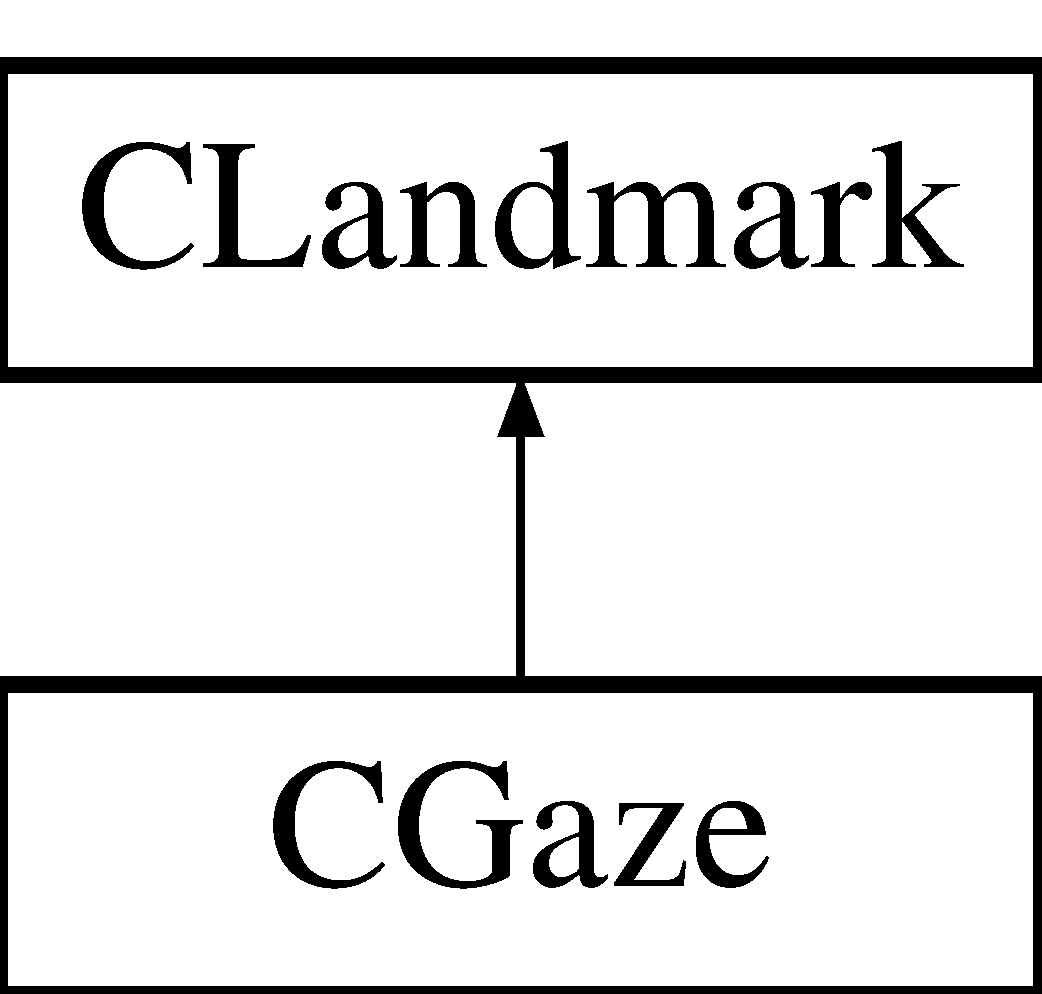
\includegraphics[height=2.000000cm]{class_c_landmark}
\end{center}
\end{figure}
\subsection*{Public Member Functions}
\begin{DoxyCompactItemize}
\item 
\mbox{\Hypertarget{class_c_landmark_a2dceda1ec703ddb81f460a73d8bb97cf}\label{class_c_landmark_a2dceda1ec703ddb81f460a73d8bb97cf}} 
{\bfseries C\+Landmark} (\hyperlink{class_c_landmark_candidate}{C\+Landmark\+Candidate} \&candidate, const char $\ast$sz\+Window)
\item 
\mbox{\Hypertarget{class_c_landmark_a1c753bf659bf8b4dbd2b7f118193fa65}\label{class_c_landmark_a1c753bf659bf8b4dbd2b7f118193fa65}} 
void {\bfseries Draw} (\hyperlink{class_c_image}{C\+Image} \&img)
\end{DoxyCompactItemize}
\subsection*{Static Public Member Functions}
\begin{DoxyCompactItemize}
\item 
\mbox{\Hypertarget{class_c_landmark_ad601efa5dbb5955f99b69901bbcac77e}\label{class_c_landmark_ad601efa5dbb5955f99b69901bbcac77e}} 
static std\+::vector$<$ \hyperlink{class_c_landmark}{C\+Landmark} $>$ {\bfseries Get\+Landmarks} (\hyperlink{class_c_image}{C\+Image} \&img, const char $\ast$sz\+Window)
\item 
\mbox{\Hypertarget{class_c_landmark_a1666a626e9533609b2810299992115b7}\label{class_c_landmark_a1666a626e9533609b2810299992115b7}} 
static std\+::vector$<$ \hyperlink{class_c_landmark}{C\+Landmark} $>$ {\bfseries Get\+Landmarks} (std\+::vector$<$ \hyperlink{class_c_landmark_candidate}{C\+Landmark\+Candidate} $>$ vec\+Candidates, const char $\ast$sz\+Window)
\end{DoxyCompactItemize}
\subsection*{Data Fields}
\begin{DoxyCompactItemize}
\item 
\mbox{\Hypertarget{class_c_landmark_a5a820e77c5e5a2158f01ecd21efc751e}\label{class_c_landmark_a5a820e77c5e5a2158f01ecd21efc751e}} 
\hyperlink{class_c_b_box}{C\+B\+Box} {\bfseries box\+Face}
\item 
\mbox{\Hypertarget{class_c_landmark_a4af2672b6cbb2ae5ed409d23893967b9}\label{class_c_landmark_a4af2672b6cbb2ae5ed409d23893967b9}} 
\hyperlink{class_c_point}{C\+Point} {\bfseries pt\+Eye\+Left}
\item 
\mbox{\Hypertarget{class_c_landmark_a3ad9329a7cefaa517fe0f111fec76f05}\label{class_c_landmark_a3ad9329a7cefaa517fe0f111fec76f05}} 
\hyperlink{class_c_point}{C\+Point} {\bfseries pt\+Eye\+Right}
\item 
\mbox{\Hypertarget{class_c_landmark_add67bd1af83f5740f67016cd3722fde7}\label{class_c_landmark_add67bd1af83f5740f67016cd3722fde7}} 
\hyperlink{class_c_point}{C\+Point} {\bfseries pt\+Nose}
\item 
\mbox{\Hypertarget{class_c_landmark_aa8dd09c2d060ddea585e38a0b5a480cf}\label{class_c_landmark_aa8dd09c2d060ddea585e38a0b5a480cf}} 
double {\bfseries d\+Distance}
\end{DoxyCompactItemize}


The documentation for this class was generated from the following files\+:\begin{DoxyCompactItemize}
\item 
D\+:/\+Users/\+Rainer/\+Source/\+Repos/deep\+\_\+learning/gaze\+\_\+data/Landmark.\+h\item 
D\+:/\+Users/\+Rainer/\+Source/\+Repos/deep\+\_\+learning/gaze\+\_\+data/Landmark.\+cpp\end{DoxyCompactItemize}

\hypertarget{class_c_landmark_candidate}{}\section{C\+Landmark\+Candidate Class Reference}
\label{class_c_landmark_candidate}\index{C\+Landmark\+Candidate@{C\+Landmark\+Candidate}}
\subsection*{Public Member Functions}
\begin{DoxyCompactItemize}
\item 
\mbox{\Hypertarget{class_c_landmark_candidate_ad7c89dce9fd8e5bdbe805b6c76f3ef1f}\label{class_c_landmark_candidate_ad7c89dce9fd8e5bdbe805b6c76f3ef1f}} 
{\bfseries C\+Landmark\+Candidate} (const \hyperlink{class_c_b_box}{C\+B\+Box} \&box\+Face)
\item 
\mbox{\Hypertarget{class_c_landmark_candidate_a00058230e636bee08a13adda9ab20325}\label{class_c_landmark_candidate_a00058230e636bee08a13adda9ab20325}} 
{\bfseries C\+Landmark\+Candidate} (const \hyperlink{class_c_landmark_candidate}{C\+Landmark\+Candidate} \&other)
\item 
\mbox{\Hypertarget{class_c_landmark_candidate_ab16bfdd8190d18934fbeb9dce3fba5d7}\label{class_c_landmark_candidate_ab16bfdd8190d18934fbeb9dce3fba5d7}} 
void {\bfseries Draw} (\hyperlink{class_c_image}{C\+Image} \&img)
\end{DoxyCompactItemize}
\subsection*{Static Public Member Functions}
\begin{DoxyCompactItemize}
\item 
\mbox{\Hypertarget{class_c_landmark_candidate_a74e87c2e505868922652bbc44fe16817}\label{class_c_landmark_candidate_a74e87c2e505868922652bbc44fe16817}} 
static std\+::vector$<$ \hyperlink{class_c_landmark_candidate}{C\+Landmark\+Candidate} $>$ {\bfseries Get\+Candidates} (\hyperlink{class_c_image}{C\+Image} \&img)
\item 
\mbox{\Hypertarget{class_c_landmark_candidate_a4ef45ae7cdc9bf64dda58a3a633188d8}\label{class_c_landmark_candidate_a4ef45ae7cdc9bf64dda58a3a633188d8}} 
static void {\bfseries Init} (void)
\end{DoxyCompactItemize}
\subsection*{Data Fields}
\begin{DoxyCompactItemize}
\item 
\mbox{\Hypertarget{class_c_landmark_candidate_a3e7f2980b5aa2391887a895e54095d7a}\label{class_c_landmark_candidate_a3e7f2980b5aa2391887a895e54095d7a}} 
\hyperlink{class_c_b_box}{C\+B\+Box} {\bfseries box\+Face}
\item 
\mbox{\Hypertarget{class_c_landmark_candidate_a18d3fb522bdfec99bd15c4af8b92941a}\label{class_c_landmark_candidate_a18d3fb522bdfec99bd15c4af8b92941a}} 
std\+::deque$<$ \hyperlink{class_c_b_box}{C\+B\+Box} $>$ {\bfseries a\+Eyes}
\item 
\mbox{\Hypertarget{class_c_landmark_candidate_a42a62cdec3aeb26cf865cad16bc9b357}\label{class_c_landmark_candidate_a42a62cdec3aeb26cf865cad16bc9b357}} 
std\+::deque$<$ \hyperlink{class_c_b_box}{C\+B\+Box} $>$ {\bfseries a\+Nose}
\end{DoxyCompactItemize}
\subsection*{Static Private Attributes}
\begin{DoxyCompactItemize}
\item 
\mbox{\Hypertarget{class_c_landmark_candidate_ab0631d51dcc7b72619bf32373bbdc58c}\label{class_c_landmark_candidate_ab0631d51dcc7b72619bf32373bbdc58c}} 
static cv\+::\+Cascade\+Classifier {\bfseries s\+\_\+\+Face\+Cascade}
\item 
\mbox{\Hypertarget{class_c_landmark_candidate_aec8d39f6402507d22b9e4df0f4da5fb7}\label{class_c_landmark_candidate_aec8d39f6402507d22b9e4df0f4da5fb7}} 
static cv\+::\+Cascade\+Classifier {\bfseries s\+\_\+\+Eye\+Cascade}
\item 
\mbox{\Hypertarget{class_c_landmark_candidate_a7334544231cedee6e25eba4ab946b983}\label{class_c_landmark_candidate_a7334544231cedee6e25eba4ab946b983}} 
static cv\+::\+Cascade\+Classifier {\bfseries s\+\_\+\+Nose\+Cascade}
\end{DoxyCompactItemize}


The documentation for this class was generated from the following files\+:\begin{DoxyCompactItemize}
\item 
D\+:/\+Users/\+Rainer/\+Source/\+Repos/deep\+\_\+learning/gaze\+\_\+data/Landmark\+Candidate.\+h\item 
D\+:/\+Users/\+Rainer/\+Source/\+Repos/deep\+\_\+learning/gaze\+\_\+data/Landmark\+Candidate.\+cpp\end{DoxyCompactItemize}

\hypertarget{class_c_point}{}\section{C\+Point Class Reference}
\label{class_c_point}\index{C\+Point@{C\+Point}}
Inheritance diagram for C\+Point\+:\begin{figure}[H]
\begin{center}
\leavevmode
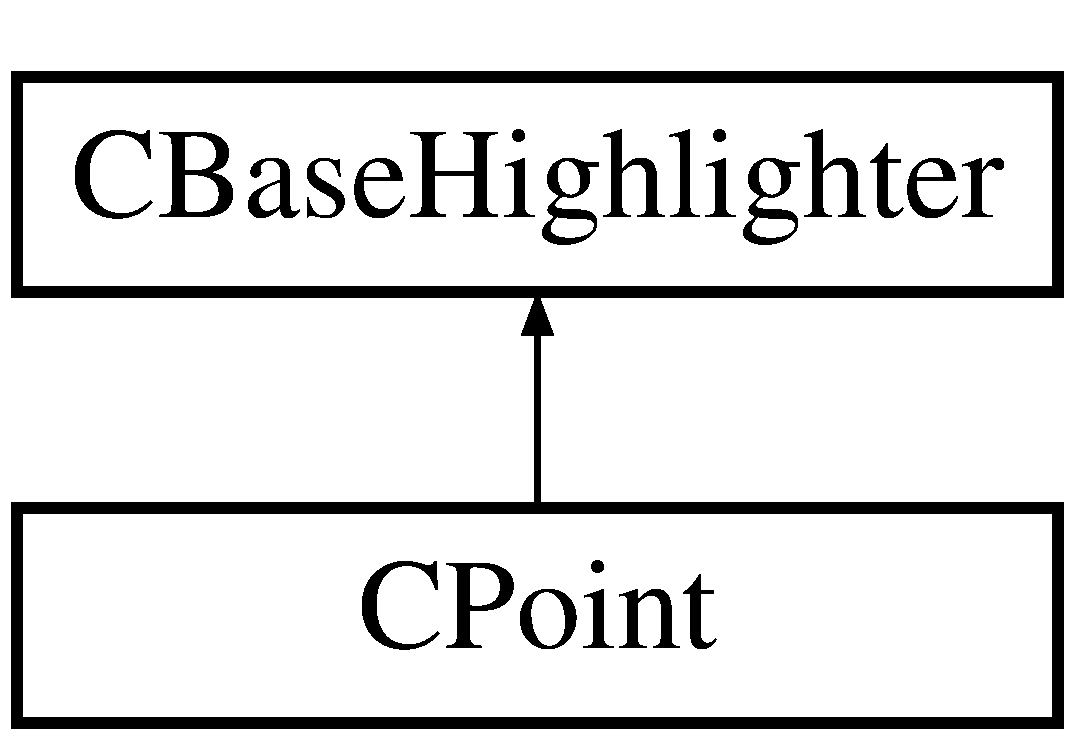
\includegraphics[height=2.000000cm]{class_c_point}
\end{center}
\end{figure}
\subsection*{Public Member Functions}
\begin{DoxyCompactItemize}
\item 
\mbox{\Hypertarget{class_c_point_aef3d46bf07181f0161b630c54263b8d5}\label{class_c_point_aef3d46bf07181f0161b630c54263b8d5}} 
{\bfseries C\+Point} (\hyperlink{class_c_base_b_box}{C\+Base\+B\+Box} \&parent\+Box, const cv\+::\+Point \&point, unsigned int u\+Level, const char $\ast$sz\+Name)
\item 
\mbox{\Hypertarget{class_c_point_a762079d20961a8be6ede2d28018be7a5}\label{class_c_point_a762079d20961a8be6ede2d28018be7a5}} 
{\bfseries C\+Point} (\hyperlink{class_c_base_b_box}{C\+Base\+B\+Box} \&parent\+Box, double d\+PositionX, double d\+PositionY, const char $\ast$sz\+Name)
\item 
\mbox{\Hypertarget{class_c_point_a12f674d0a9d500b148949a55e9a49581}\label{class_c_point_a12f674d0a9d500b148949a55e9a49581}} 
{\bfseries C\+Point} (const \hyperlink{class_c_point}{C\+Point} \&other)
\item 
\mbox{\Hypertarget{class_c_point_a3f75d6f3019610e56b5521f19586f63b}\label{class_c_point_a3f75d6f3019610e56b5521f19586f63b}} 
void {\bfseries Swap} (\hyperlink{class_c_point}{C\+Point} \&other, bool f\+Swap\+Children=true)
\item 
\mbox{\Hypertarget{class_c_point_a68f64d65a92847f3cbf949f94a2d3d10}\label{class_c_point_a68f64d65a92847f3cbf949f94a2d3d10}} 
\hyperlink{class_c_point}{C\+Point} \& {\bfseries operator=} (const \hyperlink{class_c_point}{C\+Point} \&other)
\item 
\mbox{\Hypertarget{class_c_point_a7c2762d29e6f01a75bec57b8c0a400ef}\label{class_c_point_a7c2762d29e6f01a75bec57b8c0a400ef}} 
void {\bfseries Draw} (const cv\+::\+Scalar \&color, int i\+Radius=1, int i\+Thickness=-\/1, unsigned int u\+Level=-\/1)
\item 
\mbox{\Hypertarget{class_c_point_a8a9eab0b48d20229d997c0354f32b21c}\label{class_c_point_a8a9eab0b48d20229d997c0354f32b21c}} 
void {\bfseries Draw} (\hyperlink{class_c_image}{C\+Image} \&img, const cv\+::\+Scalar \&color, int i\+Radius=1, int i\+Thickness=-\/1)
\end{DoxyCompactItemize}
\subsection*{Additional Inherited Members}


The documentation for this class was generated from the following files\+:\begin{DoxyCompactItemize}
\item 
D\+:/\+Users/\+Rainer/\+Source/\+Repos/deep\+\_\+learning/gaze\+\_\+data/Point.\+h\item 
D\+:/\+Users/\+Rainer/\+Source/\+Repos/deep\+\_\+learning/gaze\+\_\+data/Point.\+cpp\end{DoxyCompactItemize}

%--- End generated contents ---

% Index
\backmatter
\newpage
\phantomsection
\clearemptydoublepage
\addcontentsline{toc}{chapter}{Index}
\printindex

\end{document}
